\pdfoutput=1
\documentclass[aps,pra,reprint,superscriptaddress,nofootinbib,longbibliography,floatfix]{revtex4-2}

\usepackage[T1]{fontenc}
\usepackage{lmodern}
\usepackage{amsmath,amssymb}
\usepackage{upgreek}
\usepackage{graphicx}
\usepackage{xcolor}
\usepackage[colorlinks=true,linkcolor=blue!50!black,citecolor=blue!50!black,urlcolor=blue!50!black]{hyperref}
\hypersetup{
  pdftitle={Distance scaling of the heavy-hex subsystem code on IBM Fez: a pre-registered test of a calibration-based noise model},
  pdfauthor={Nadav Abramson}
}

\newcommand{\ket}[1]{\lvert #1\rangle}
\newcommand{\eps}{\varepsilon}
\newcommand{\us}{\,\upmu\mathrm{s}}
\newcommand{\LX}{\Lambda_{\mathrm{X}}}
\newcommand{\LZ}{\Lambda_{\mathrm{Z}}}

\begin{document}

\title{\texorpdfstring{Distance scaling of the heavy-hex subsystem code on IBM Fez:\\ a pre-registered test of a calibration-based noise model}{Distance scaling of the heavy-hex subsystem code on IBM Fez: a pre-registered test of a calibration-based noise model}}

\author{Nadav Abramson}
\affiliation{Independent researcher}
% \email{}  % add a contact address and city/country before submission

\date{October 9, 2026}

\begin{abstract}
We report a pre-registered memory experiment with the heavy-hex subsystem code at distances 3 and 5 on IBM's 156-qubit Heron~r2 processor \texttt{ibm\_fez}, designed to test whether a circuit-level noise model built from IBM's published calibration predicts logical error rates.
Placement, circuits, analysis and decision rules were fixed in code before the first job, and before each job we committed its calibration, compiled circuits and model predictions bracketing the one parameter the calibration does not supply, which the same job then measured.
Over ten repetitions on five days, on the only two distance-5 placements usable each day, the distance-5 patch fails more often than the distance-3 patch in X memory in 59 of 60 pairs of repetition and round count, the sixtieth being a tie within one shot in 2500.
The error-suppression factor is $\LX = 0.68\pm0.03$ and $0.50\pm0.02$ on the two placements, against $0.64$ and $0.45$ predicted.
The model nevertheless fails the pre-registered agreement test: it underestimates the logical error per round by 14--28\% in X memory and by a factor of 1.6--1.9 in Z memory, and matches $\LX$ only after a post hoc allowance for day-to-day scatter in the calibration.
Flag and relay qubits, which should read zero, reveal the largest discrepancy we can identify: a hidden state that survives the measure-and-flip reset for about $30\us$, randomizes the readout and is shared by neighbouring qubits, as leakage out of the computational subspace would.
A leakage-aware simulation fitted to detection statistics alone closes a third to a half of the Z-memory gap.
\end{abstract}

\maketitle

%======================================================================
\section{Introduction}
%======================================================================

Quantum error correction pays off only if enlarging a code lowers its logical error rate.
The standard figure of merit is the error-suppression factor
\begin{equation}
  \Lambda = \eps_3 / \eps_5 ,
  \label{eq:lambda}
\end{equation}
the ratio of the logical error per round at code distances 3 and 5; the larger code is better when $\Lambda > 1$~\cite{google2023suppressing,google2025below}.
Google's surface code reached $\Lambda \approx 1.04$ on Sycamore~\cite{google2023suppressing} and $\Lambda = 2.14 \pm 0.02$ on Willow~\cite{google2025below}.
On IBM's square-lattice Nighthawk processor, a distance-5 surface code recently reached $0.98\%$ per round against $1.26\%$ at distance~3 in Z memory, with defective components excluded and leaked shots post-selected away~\cite{drouet2026error}.

IBM's Heron processors instead use a heavy-hex lattice, in which no qubit has more than three neighbours.
The heavy-hex subsystem code was designed for this connectivity~\cite{chamberland2020topological}, using flag qubits~\cite{chao2018quantum} to measure its weight-four gauge operators.
It has been run at distance~3 on a 27-qubit Falcon processor~\cite{sundaresan2023demonstrating} and on Heron~r2~\cite{harper2026characterising}, and at distance~5 on Heron~r3 in an appendix of a study of the dynamic compass code~\cite{lee2026scalable}.
Other codes embedded in heavy-hex hardware have generally performed worse at larger distance~\cite{hall2024artificial,hetenyi2024creating}.
A SWAP-embedded surface code reached $\Lambda \approx 1.2$--$1.5$ in the basis protected by its enlarged distance, though only 1.0--1.1 against its best distance-3 sub-patch and $0.67$--$0.77$ averaged over bases~\cite{vezvaee2026surface}, and a comparative study found such embeddings more promising than the native heavy-hex code~\cite{benito2025comparative}.

On hardware of this quality, whether $\Lambda$ exceeds one is hardly in question: simulations from the device calibration place it below one before any data are taken (Sec.~\ref{sec:prerun}).
The more useful question is whether such simulations get the numbers right.
Calibration-based models have repeatedly mispredicted IBM hardware: a Stim model underestimated errors on Nighthawk~\cite{drouet2026error}, one overestimated distance-3 errors in Ref.~\cite{hall2024artificial}, reproducing Heron data required fitted reset and readout errors~\cite{harper2026characterising}, and on \texttt{ibm\_sherbrooke} a single error rate fitted to detector statistics predicted logical errors better than per-qubit benchmarks~\cite{hesner2025using}.
These comparisons were made after the data were in hand.
In quantum-error-correction experiments many analysis choices---where to place the code, which shots to post-select, which decoder priors and which range of rounds to fit---can move $\Lambda$ by more than its statistical error, which makes a prospective test informative.

Here we test a calibration-based model prospectively.
We ran the heavy-hex code at distances 3 and 5 on \texttt{ibm\_fez} on five days, placing the patches each day from IBM's latest calibration and committing, before each job, the circuits, the calibration and the model's predictions.
The only model input the calibration does not supply, the dephasing left by our dynamical-decoupling pulses, is measured by idle circuits in the same job.
The model reproduces the ordering and approximate size of $\LX$ on the two placements, but underestimates the logical error rates and fails the pre-registered agreement test.
An exploratory analysis of the flag and relay readouts points to leakage as the largest identifiable cause.
No shots were post-selected or discarded at any stage.

%======================================================================
\section{Code and circuits}
\label{sec:code}
%======================================================================

The $[[d^2,1,d]]$ heavy-hex code is a hybrid: it corrects Z errors as a surface code and X errors as a Bacon--Shor code~\cite{bacon2006operator}; we follow the labels of Ref.~\cite{sundaresan2023demonstrating}, while Ref.~\cite{chamberland2020topological} exchanges X and Z.
Its gauge group is generated by weight-2 X gauges and by weight-4 bulk and weight-2 edge Z gauges.
Each weight-4 X stabilizer is the product of two X gauges, and each weight-2 edge X stabilizer is a single gauge; these form the surface-code half, in which below a threshold a larger patch corrects more.
Each Z stabilizer is the product of the Z gauges along a pair of columns and has weight $2d$; with the same gauges measured every round, this Bacon--Shor half has no threshold~\cite{chamberland2020topological,napp2013optimal}, because a larger patch's stabilizers accumulate more errors per round.
X memory fails only through Z errors and is therefore the test of scaling; Z memory fails through X errors and serves mainly as a test of the noise model.
Table~\ref{tab:code} lists the resources at each distance.

\begin{table}[b]
\caption{The two patches.}
\label{tab:code}
\begin{ruledtabular}
\begin{tabular}{lcc}
 & $d=3$ & $d=5$ \\
\hline
Data qubits & 9 & 25 \\
Qubits used (with ancillas and relays) & 23 & 65 \\
X stabilizers, weight 4 + weight 2 & 2 + 2 & 8 + 4 \\
Z stabilizers, weight $2d$ & 2 & 4 \\
Readouts per round & 18 & 56 \\
\end{tabular}
\end{ruledtabular}
\end{table}

Each round measures all gauges of the memory basis, then all gauges of the other basis.
Because gauges of the same type are measured in parallel, a round lasts $7.9\us$ at both distances.
An X gauge is measured with one ancilla and two CNOT (CX) gates.
A bulk Z gauge acts on four data qubits that its ancilla cannot reach on heavy-hex; it borrows the two neighbouring X ancillas, which carry the parities of their data pairs to the Z ancilla one data qubit at a time and are then uncomputed (Fig.~\ref{fig:gadget}).
Following Refs.~\cite{chamberland2020topological,sundaresan2023demonstrating} we call these borrowed qubits flags.
Unlike flags in flag fault tolerance, their outcomes are not needed to catch high-weight errors: with the CX order used, a single fault spreads to at most one data qubit, or to two in the same column, neither of which reduces the distance.
In Z memory their outcomes, ideally 0, serve as additional detectors.
Edge Z gauges reach their data through relay qubits~\cite{chamberland2020topological,sundaresan2023demonstrating}, which are likewise uncomputed and serve as detectors.
Stim~\cite{gidney2021stim} finds circuit distance 3 and 5 in both bases for the circuits that were run, so minimum-weight matching reaches full distance without flag-conditioned decoding.

\begin{figure}[t]
\centering
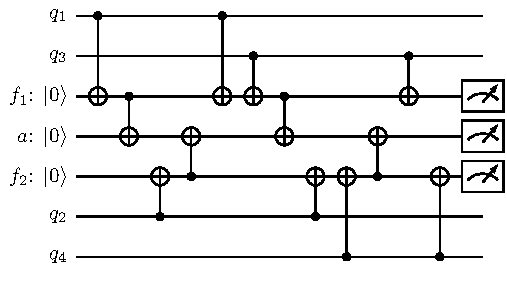
\includegraphics[width=\columnwidth]{figures/gadget.pdf}
\caption{Measurement of a bulk Z gauge $Z_{q_1}Z_{q_2}Z_{q_3}Z_{q_4}$ through the neighbouring X ancillas $f_1$, $f_2$ (flags) and the Z ancilla $a$, as executed (twelve CX gates, left to right).
Each flag copies one data qubit, passes it to $a$, swaps in the second data qubit of its pair, passes again and is uncomputed, so that it ends in $\ket{0}$ unless an X fault hit it.
Each CX is compiled as H$\cdot$CZ$\cdot$H on its target.}
\label{fig:gadget}
\end{figure}

\paragraph*{Detectors and decoding.}
Each detector compares a stabilizer's value with its value in the previous round.
In the first round, memory-basis stabilizers are compared with their deterministic initial value, and other-basis stabilizers with a reference obtained by measuring the other-basis gauges once before the first round.
A final layer of detectors compares the memory-basis stabilizers with their values reconstructed from the data readout.
In Z memory every flag and relay readout is an additional detector.
Only memory-basis detectors enter the decoder, which is minimum-weight perfect matching~\cite{higgott2025sparse} on the detector error model that Stim derives from the same circuit and noise model (Sec.~\ref{sec:model}).

\paragraph*{Compilation and timing.}
The circuits are compiled to Fez's native gates (CZ, $\sqrt{X}$, $X$ and virtual $R_Z$), and every idle period is written as an explicit delay.
Gates start as soon as their qubits are free, except resets, which are scheduled immediately before the qubit is next used.%
\footnote{Qiskit's default as-late-as-possible scheduling would postpone the closing H of each CX past the following delay, leaving data qubits in a rotated basis during readout.}
Data qubits spend $6.7\us$ of each round idle while ancillas are read out ($1.66\us$) and reset ($1.68\us$), each twice per round.
Every idle period of $500$\,ns or more receives two $X$ pulses, at one and three quarters of its length~\cite{viola1999dynamical,ezzell2023dynamical}.
IBM's own decoupling and Pauli twirling are disabled, so that the device executes exactly the circuit we simulate.

%======================================================================
\section{Placement and schedule}
\label{sec:design}
%======================================================================

A distance-3 patch fits on Fez in 30 placements and a distance-5 patch in 12, each in two orientations.
Each day, every placement that uses a part IBM marks as faulty, reports at $\ge 50\%$ error, or reports without $T_1$ or $T_2$ is discarded; the remaining placements are called clean.
Working but weak parts (CZ error above 1\%, readout error above 5\%, $T_1 < 50\us$ or $T_2 < 30\us$) are kept and listed.
Placements are scored by the summed CZ, readout and reset errors of one round and the $T_1$ decay of the data qubits.
Each day's calibration defines up to two repetitions, one per clean distance-5 placement, best first.
Each repetition's distance-3 patch takes the best clean placement not yet used that day: beside the distance-5 patch in the same job where one fits, otherwise in a separate job submitted immediately after.

\begin{figure*}[t]
\centering
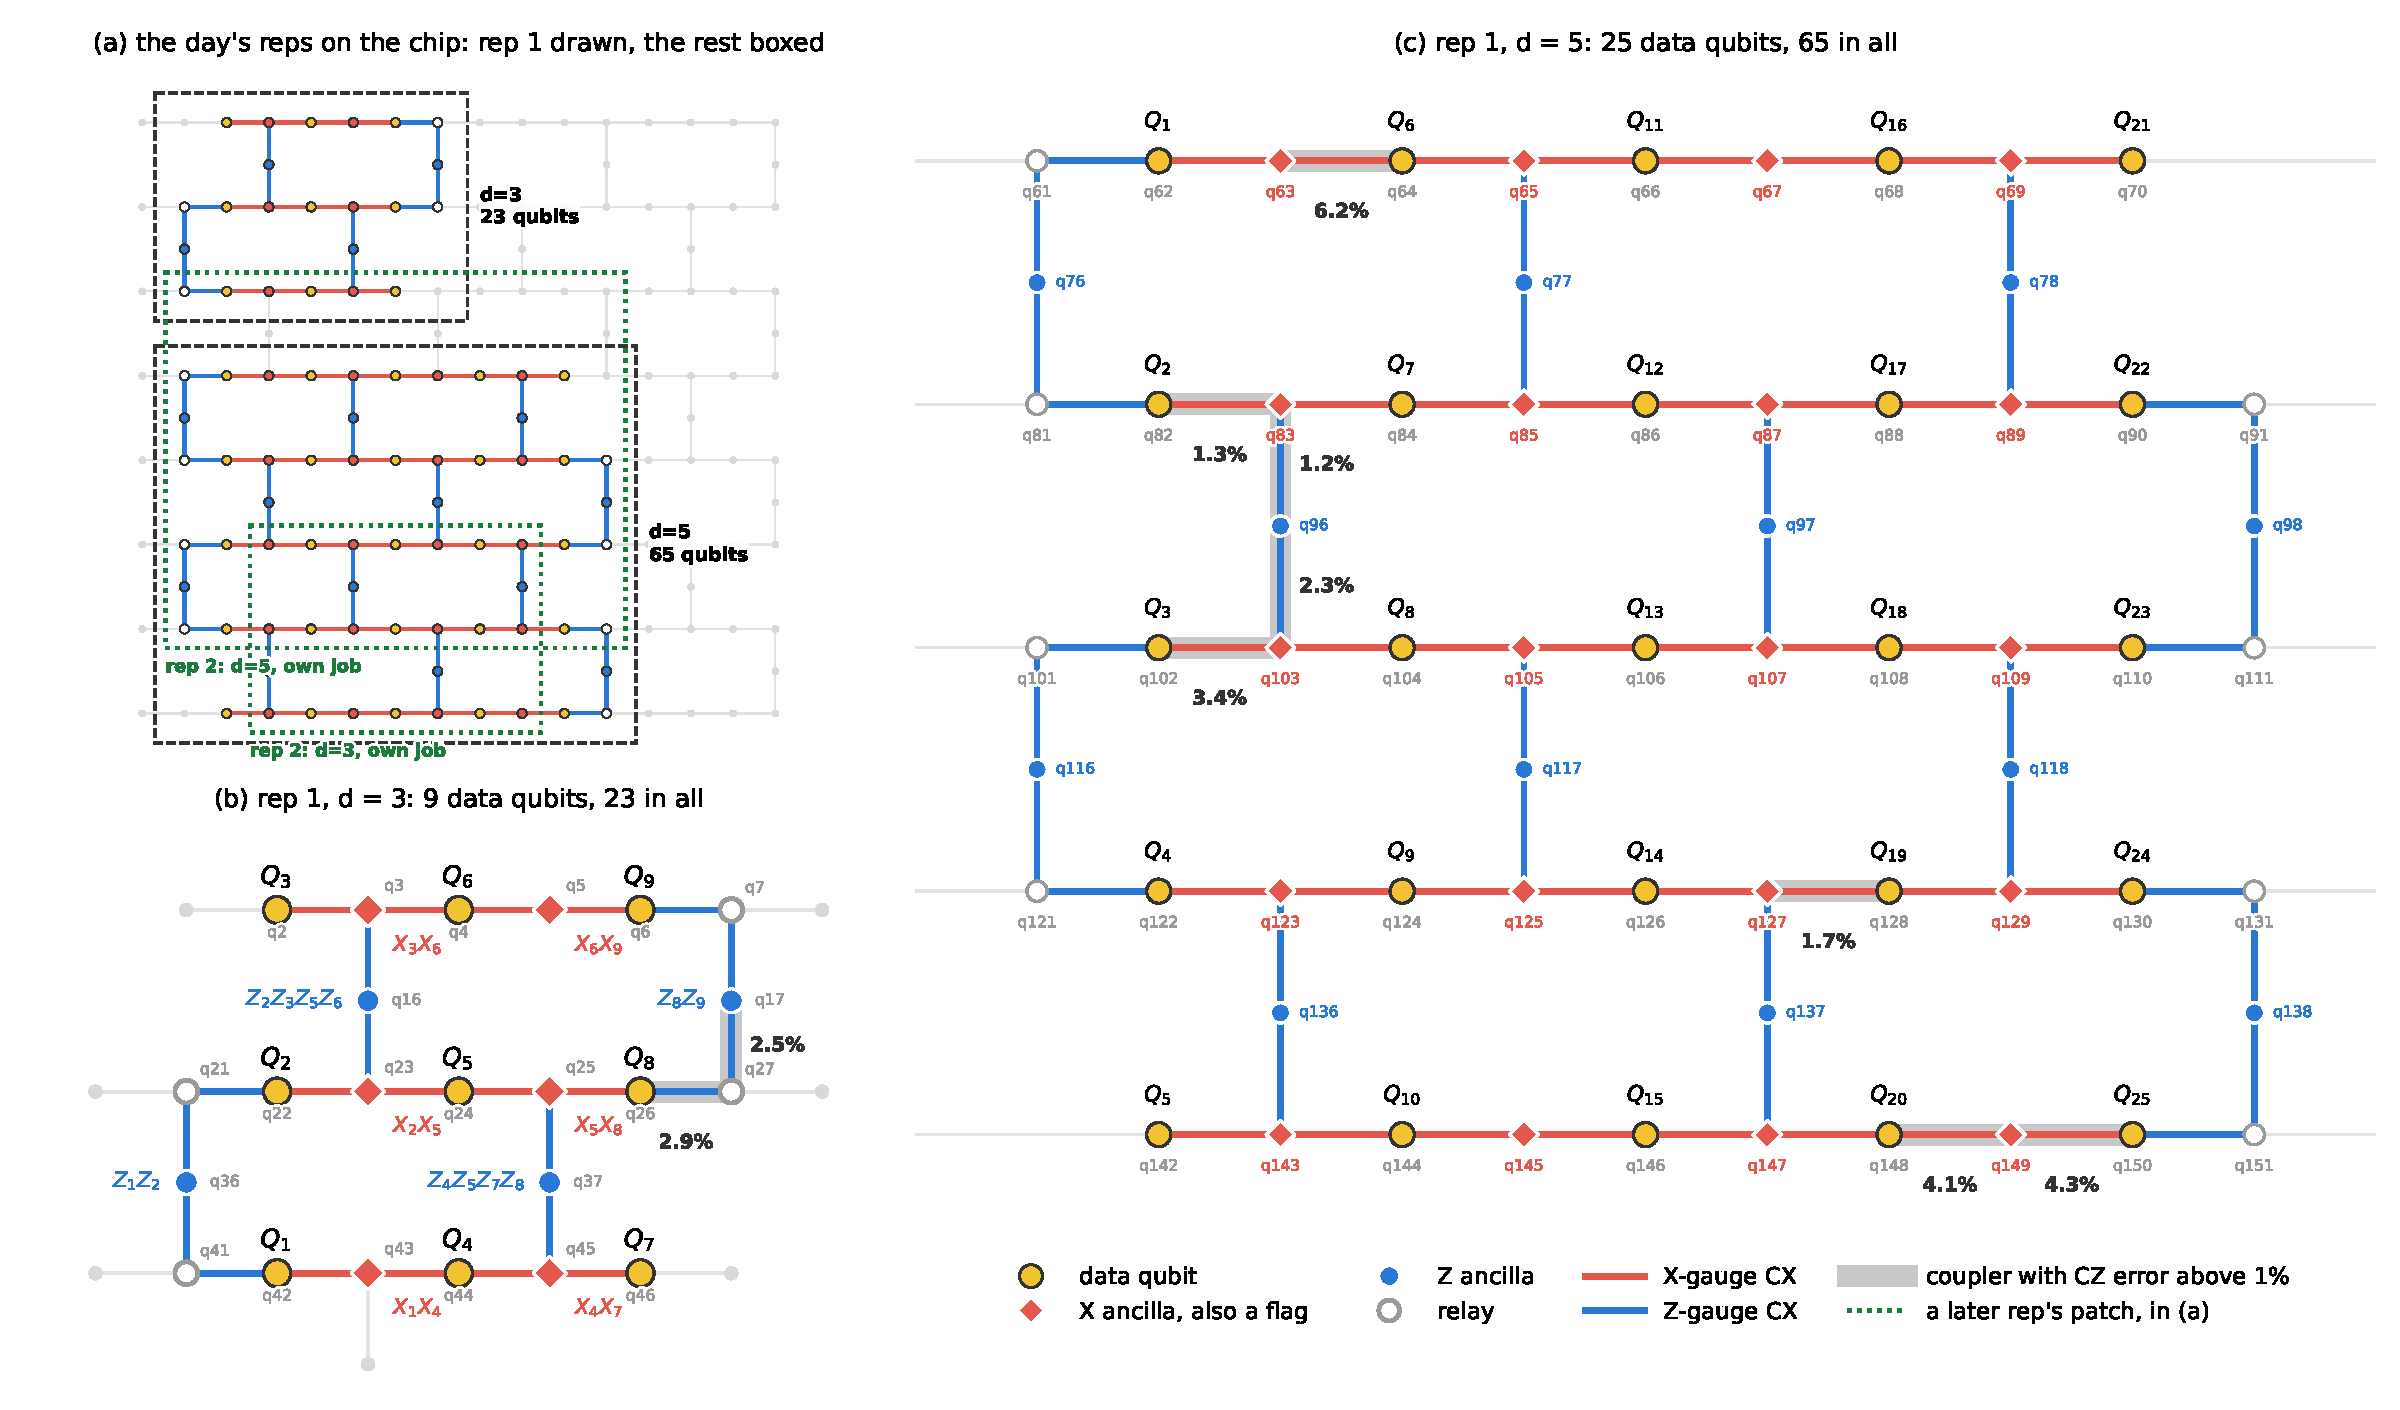
\includegraphics[width=\textwidth]{figures/layout.pdf}
\caption{The two repetitions planned on IBM's calibration of 3 October 2026, 20:05~UTC (day~1).
(a) Placement on the chip: repetition~1 drawn, repetition~2's patches boxed.
(b) Repetition~1's distance-3 patch and (c) its distance-5 patch; $Q$ labels mark data qubits and $q$ numbers Fez qubits.
Shaded couplers have CZ error above 1\%.
The same two distance-5 placements were the only clean ones on every day.}
\label{fig:layout}
\end{figure*}

On every day exactly two distance-5 placements were clean, and they share 51 of their 65 qubits (Fig.~\ref{fig:layout}).
Repetition~1 therefore ran both patches in one job.
For repetition~2 no clean distance-3 placement fitted beside the distance-5 patch, so its distance-3 patch ran about one minute later on the best clean placement on the chip; it occupied three different placements over the five days, all within repetition~1's distance-5 patch.
Each job contains X- and Z-memory circuits at $n = 1, 2, 3, 4, 6$ and $8$ rounds (2500 shots each) and ten idle-test circuits (Sec.~\ref{sec:model}; 1250 shots each).
Fifteen jobs ran on five days (Table~\ref{tab:days}), each charged 15\,s of QPU time, for a total of 225\,s against a pre-set budget of 300\,s.
IBM did not recalibrate during any job.

\begin{table*}[t]
\caption{The five run days. Chip medians over working parts from the calibration each day's jobs were prepared from, and the dephasing parameter $f$ measured in each day's three jobs.}
\label{tab:days}
\begin{ruledtabular}
\begin{tabular}{cccccccc}
Day & Jobs (UTC) & Calibration (UTC) & CZ error & Readout error & $T_1$ ($\upmu$s) & $T_2$ ($\upmu$s) & $f$ \\
\hline
1 & 3 Oct, 21:33--21:36 & 3 Oct, 20:05 & 0.27\% & 1.03\% & 132 & 104 & 0.88--1.06 \\
2 & 5 Oct, 18:05--18:09 & 5 Oct, 17:42 & 0.27\% & 1.01\% & 119 & 88 & 0.72--0.94 \\
3 & 6 Oct, 18:03--18:07 & 6 Oct, 17:41 & 0.27\% & 1.01\% & 126 & 87 & 1.05--1.52 \\
4 & 7 Oct, 17:23--17:26 & 7 Oct, 17:01 & 0.27\% & 1.02\% & 132 & 99 & 1.01--1.10 \\
5 & 8 Oct, 17:34--17:38 & 8 Oct, 17:13 & 0.27\% & 1.04\% & 122 & 87 & 0.79--0.99 \\
\end{tabular}
\end{ruledtabular}
\end{table*}

%======================================================================
\section{Noise model and pre-registered analysis}
\label{sec:model}
%======================================================================

\subsection{Model}

Each prediction is a Stim simulation of the exact compiled circuits, gate by gate and delay by delay.
Each CZ receives two-qubit depolarizing noise at $5/4$ of IBM's reported error for its coupler, and each $\sqrt{X}$ and $X$ one-qubit depolarizing noise at $3/2$ of the qubit's reported error.
These factors convert an average gate infidelity into a depolarizing probability; IBM's per-coupler CZ errors are average gate errors from randomized benchmarking that include a layer of single-qubit Cliffords~\cite{ibmdocs}.
Each measurement and reset flips with the qubit's reported readout error.
A delay of length $t$ is the Pauli-twirled amplitude- and phase-damping channel~\cite{ghosh2012surface},
\begin{equation}
\begin{aligned}
p_x = p_y &= \tfrac14\bigl(1-e^{-t/T_1}\bigr), \\
p_z &= \tfrac12\bigl(1-e^{-t/T_2}\bigr) - \tfrac14\bigl(1-e^{-t/T_1}\bigr),
\end{aligned}
\label{eq:idle}
\end{equation}
with $T_2 \le 2T_1$ and no decay for qubits resting in $\ket{0}$.
In a decoupled delay $T_2$ is replaced by
\begin{equation}
\frac{1}{T_2^{\mathrm{DD}}} = \frac{1}{2T_1} + f\left(\frac{1}{T_2}-\frac{1}{2T_1}\right),
\label{eq:f}
\end{equation}
where $f$ is the pure-dephasing rate left by the pulses in units of the rate implied by IBM's Hahn-echo $T_2$: $f=0$ leaves only $T_1$ decay and $f=1$ recovers echo dephasing.
Leakage, crosstalk, coherent errors and drift are not modelled.

The parameter $f$ is the model's one input not supplied by the calibration.
Each job measures it with ten idle circuits: X-memory circuits in which every CZ is replaced by a delay of equal length, read out in X and in Y, so that a frequency offset, which rotates X into Y, cannot mimic dephasing (Appendix~\ref{app:f}).
Before each job we committed predictions at $f=0$ and $f=1$, which bracket the expected range.
The prediction that is tested evaluates the committed model, circuits and calibration at the median $f$ measured by the same job, with the code version recorded before the job.

\subsection{Decision rules}

For each patch and basis, the logical error $P(n)$ after $n$ rounds is fitted as $1-2P(n) = A(1-2\eps)^n$ by weighted least squares on $\ln[1-2P(n)]$, omitting points with $P(n)\ge 0.5$; $A$ absorbs preparation, readout and time-boundary effects.
For each repetition, distance~5 is declared better (worse) if $\LX - 1.645\sigma > 1$ ($\LX + 1.645\sigma < 1$); otherwise the result is undecided.
The experiment's answer is $\LX$ pooled over repetitions with inverse-variance weights; its standard error is widened by $\sqrt{\chi^2/\nu}$ when the repetitions scatter more than their errors allow, and Student's $t$ for $\nu = R-1$ degrees of freedom replaces 1.645.
The model agrees with a repetition in X memory if $\LX$, $\eps_3$ and $\eps_5$ each lie within twice the combined observed and predicted standard error of their predictions; across the experiment, the test is a $\chi^2$ sum over repetitions against its 95th percentile.
Z memory is reported but was not to be tested.
Side checks for drift within a job, for a detection rate that rises over rounds beyond the prediction (a signature of leakage or heating), and for individual detectors firing far above prediction are reported without affecting the decisions.
Appendix~\ref{app:stats} gives the details and the simulated error rates of these rules.

\subsection{Record}

The design, code and decision rules were fixed in code before the first job.
The multi-day design and the pooling rule were committed 31 and 13 minutes before that job, and the code was released as v0.2.0 and archived by Zenodo~\cite{zenodo} four minutes before it; this archive is the only third-party timestamp in the record.
Each day's calibration, compiled circuits and committed predictions were pushed to the public repository before that day's first job, and the submission software refuses a job whose folder has not been pushed.
The analysis code did not change during the experiment: all fifteen jobs record the same version.
Every planned job was run, and none was repeated or excluded.
Appendix~\ref{app:record} gives the timeline.

\subsection{What the model predicted before the run}
\label{sec:prerun}

On the calibration of day~1, the model placed $\LX$ below one for two reasons.
First, placement: the distance-5 patch must take whichever of its 12 placements is clean, and on day~1 its best placement contained a coupler with 6.2\% CZ error, a qubit with 14\% readout error and two qubits with $T_2$ of 5--6$\us$.
Placing the simulated distance-3 patch on a sub-patch of the distance-5 patch's own qubits raises $\LX$ from 0.54 to 0.65--0.70, whereas setting only the weak parts of both patches to the chip median gives 0.61--0.62.
Second, the error rates: with every CZ, readout, $T_1$ and $T_2$ at the chip median, the simulated $\LX$ is 0.94 at $f=0$ and 0.86 at $f=1$; halving the CZ error raises it to 1.10 at $f=0$.

%======================================================================
\section{Results}
\label{sec:results}
%======================================================================

\begin{figure}[t]
\centering
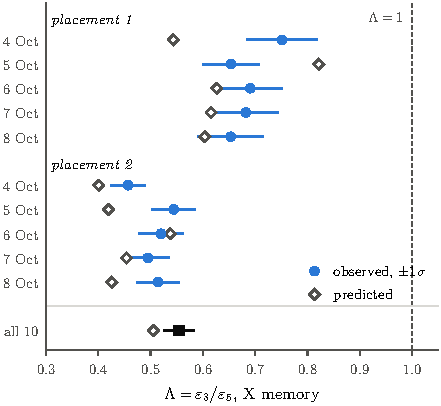
\includegraphics[width=\columnwidth]{figures/lambda.pdf}
\caption{$\LX$ for each repetition, observed (circles, $\pm1\sigma$) and predicted at the job's measured $f$ (diamonds), grouped by placement, and the value pooled over all ten repetitions with its widened error.}
\label{fig:lambda}
\end{figure}

All ten repetitions declare distance~5 worse in X memory, with $\LX$ between 0.46 and 0.75 (Fig.~\ref{fig:lambda}).
The conclusion does not depend on the fitting procedure: in X memory the distance-5 patch has the higher logical error in 59 of the 60 pairs of repetition and round count, and in the sixtieth (day~4, repetition~1, one round) the two differ by a single shot in 2500 (Fig.~\ref{fig:pn}).
Pooled over the repetitions, $\LX = 0.55 \pm 0.03$, against 0.51 predicted; after widening the error by $\sqrt{\chi^2/\nu} = 2.0$, the pooled value lies 15 standard errors below one, far beyond the critical value $t_9 = 1.83$.

\begin{figure*}[t]
\centering
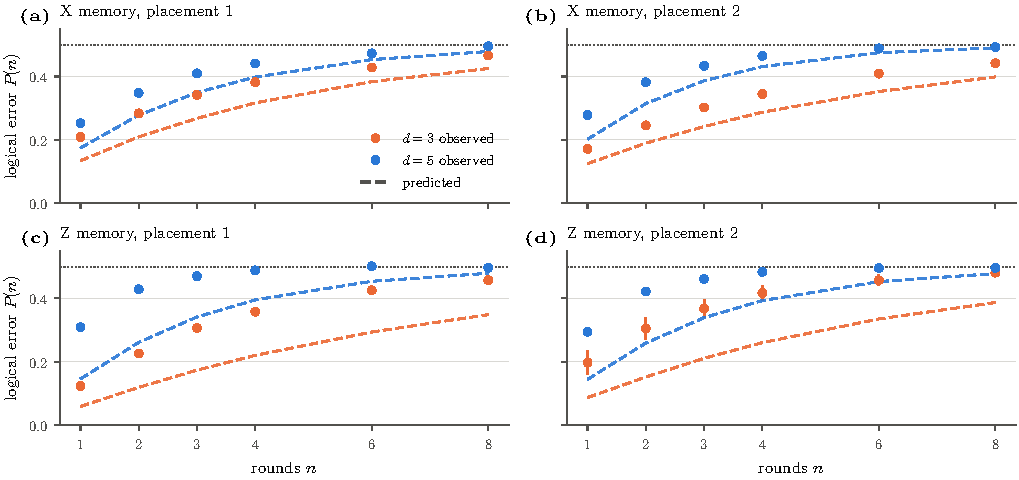
\includegraphics[width=\textwidth]{figures/pn.pdf}
\caption{Logical error $P(n)$ after $n$ rounds on each placement, mean over the five days ($\pm$ standard error over days), with the prediction at each job's measured $f$ averaged likewise (dashed).
The device exceeds the prediction from the first round; in Z memory the distance-3 error is about twice the prediction.
Distance-5 X memory approaches 50\% by six rounds.}
\label{fig:pn}
\end{figure*}

\begin{table*}[t]
\caption{Logical error per round and $\Lambda$ by placement, pooled over the five days ($\pm$ one standard error, widened as in Sec.~\ref{sec:model}), with the mean prediction at the measured $f$ and its range over the days.}
\label{tab:placement}
\begin{ruledtabular}
\begin{tabular}{llccc}
 & & $\eps_3$ (\%) & $\eps_5$ (\%) & $\Lambda$ \\
\hline
X memory, placement 1 & observed & $12.5\pm0.3$ & $18.4\pm0.5$ & $0.68\pm0.03$ \\
 & predicted & 10.2 (9.6--11.8) & 16.1 (14.3--17.9) & 0.64 (0.54--0.82) \\
X memory, placement 2 & observed & $11.0\pm0.4$ & $21.9\pm0.6$ & $0.50\pm0.02$ \\
 & predicted & 8.6 (7.7--10.2) & 19.2 (18.3--20.1) & 0.45 (0.40--0.54) \\
Z memory, placement 1 & observed & $13.7\pm0.3$ & $29.8\pm1.7$ & $0.44\pm0.03$ \\
 & predicted & 7.1 (6.2--8.2) & 16.6 (15.3--17.4) & 0.43 (0.35--0.49) \\
Z memory, placement 2 & observed & $15.6\pm1.3$ & $26.3\pm1.0$ & $0.63\pm0.05$ \\
 & predicted & 8.4 (7.7--8.8) & 16.5 (15.4--18.3) & 0.51 (0.42--0.57) \\
\end{tabular}
\end{ruledtabular}
\end{table*}

The ten repetitions are, in effect, two placements measured on five days each.
$\LX$ is $0.68\pm0.03$ on placement~1 and $0.50\pm0.02$ on placement~2 (predicted 0.64 and 0.45 on average), and within each placement the five days agree ($\chi^2/\nu = 0.4$ and $0.8$; Table~\ref{tab:placement}).
The device's $\LX$ is therefore stable from day to day, and the excess scatter between repetitions reflects placement; Z memory varies more ($\chi^2/\nu = 1.9$ and $2.7$ within placements).
Because the pooled rule treats repetitions as independent, its error bar is too narrow for a statement about the device as a whole: taking the placement as the unit ($n=2$) gives $\LX = 0.59 \pm 0.09$, which the same test leaves undecided (one-sided $p \approx 0.07$).
The conclusion that distance~5 is worse is therefore firm for these two placements, the only clean ones on every day, and suggestive for Fez in general.

Part of the gap between distances is selection.
The distance-3 patch of repetition~2 always sat on the best clean placement on the chip, while the distance-5 patch had to take one of two.
Comparing, post hoc, repetition~2's distance-3 patches, which lie within repetition~1's distance-5 patch, with that distance-5 patch gives $\eps_3/\eps_5 \approx 0.60$, against 0.50 for repetition~2 as registered.
Other estimators of the pooled value give 0.55--0.60 (Appendix~\ref{app:stats}).

%======================================================================
\section{Model versus device}
\label{sec:agreement}
%======================================================================

The model captures the ordering of the placements and the approximate size of $\LX$, but not the error rates that form it, and the pre-registered agreement test fails.
$\eps_3$ in X memory exceeds its prediction in every repetition, by 1--56\%.
Across the experiment the tests fail for $\LX$ ($\chi^2 = 25.0$ against a 95\% bound of 18.3 for ten repetitions), for $\eps_3$ (52.1) and for $\eps_5$ (19.8); four of ten repetitions agree on all three quantities and eight agree on $\LX$.
Applied post hoc to Z memory, the same test shows errors about twice the prediction at distance~3 ($\chi^2 = 1240$ for $\eps_3$, 271 for $\eps_5$, 35.2 for $\LZ$).
Because Z memory does not depend on $f$, its miss points at the calibrated CZ, readout and $T_1$ inputs or at physics outside the model.
Detector by detector the same picture holds: between 171 and 834 of the 1428 detectors in a two-patch job fire above prediction by more than $\sqrt{2\ln 1428} = 3.81$ standard errors against the calibrations both before and after the job, the largest excesses (up to 5.3 times the predicted rate) being flag detectors in Z memory.

Part of the X-memory disagreement reflects the calibration rather than the device.
On placement~1 the predicted $\LX$ moved between 0.54 and 0.82 over the five days while the measured value stayed between 0.65 and 0.75.
The pre-registered bound allows for shot noise, the uncertainty in $f$ and recalibration during a job, but not for this day-to-day scatter in IBM's numbers.
As a post hoc check, we add to each predicted quantity its relative standard deviation over the five days of predictions on placement~1 (16\% for $\LX$, 9\% for $\eps_3$, 8\% for $\eps_5$).
$\LX$ then passes ($\chi^2 = 7.8$ against 18.3), and continues to pass for any relative scatter above about 6\%.
$\eps_5$ passes marginally (13.4) and would fail with placement~2's smaller prediction scatter; $\eps_3$ (35.3) and all Z-memory tests still fail.
This treats the calibration's daily changes as noise in the prediction rather than changes of the device, an interpretation suggested, but not proven, by the device's own day-to-day stability.

Two-pulse decoupling performed no better than a Hahn echo.
The idle tests give $f$ between 0.72 and 1.52 across the fifteen jobs (median 0.99), with a spread across qubits far exceeding the per-qubit uncertainties ($\chi^2/\nu$ of 12--80 about the weighted mean in every job).
Values of $f$ read back from the memory runs agree with the idle test in ten of fifteen jobs and are higher in the other five, as expected if the idle test, which omits the CZ pulses and keeps neighbouring ancillas in $\ket{0}$, underestimates the dephasing during memory.
The detection rate rises over the rounds beyond the prediction in 25 of the 40 eight-round memory circuits, at least once in every job; drift within jobs is absent (the largest change between the first and second halves of a job's shots is 2.5$\sigma$).

%======================================================================
\section{Diagnosis: leakage}
\label{sec:leakage}
%======================================================================

The analyses in this section are exploratory: they were chosen after the run, use only the run's shots and IBM's published calibrations, and change nothing above.
They draw on the 320 readout series of flags and relays in eight-round Z memory, which come from 38 physical qubits over fifteen jobs.

\paragraph{Temporal correlations.}
In Z memory every flag and relay should read 0 in each round, and in the calibration model successive rounds are independent.
On the device, a flag or relay is 14.8 percentage points more likely to fire in a round if it fired in the previous one, and the excess decays over tens of microseconds (Fig.~\ref{fig:leak}a); the model gives zero at every lag.
The excess appears in 319 of the 320 series, and runs of five or more consecutive firings are nine times as frequent as the model allows (0.33\% of shots against 0.035\%).

\paragraph{A persistent hidden state.}
A two-state hidden Markov model, with a normal and a persistent state, fits 97\% of the series better than independent rounds (log-likelihood gain above 10, median 327), although the independent model has more free parameters (one rate per round, 18 in all, against five); it finds no such state in shots sampled from the calibration model.
The persistent state is entered in about 2.5\% of rounds, lasts about $31\us$ (four rounds), and makes the readout fire about half the time.
Outside it, flags fire in 4.1\% of rounds against the model's 4.4\%.

\begin{figure*}[t]
\centering
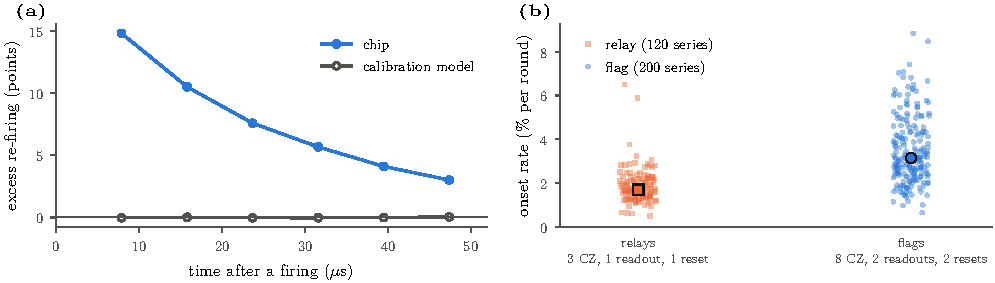
\includegraphics[width=\textwidth]{figures/leakage.pdf}
\caption{(a) Excess probability that a flag or relay fires again a given time after it fired, relative to one that did not, averaged over the 320 readout series of eight-round Z memory, for the device and for shots sampled from the calibration model.
(b) Per-series rate of entering the persistent state in a two-state hidden Markov fit, for relays and flags, with the operations each takes part in per round (horizontal jitter added); large markers are medians.}
\label{fig:leak}
\end{figure*}

\paragraph{Consistent with leakage.}
In transmon processors, leakage out of $\{\ket{0},\ket{1}\}$ arises in two-qubit gates and in measurement, persists for tens of microseconds, and spreads to neighbours through two-qubit gates~\cite{mcewen2021removing,miao2023overcoming}.
A reset that measures and conditionally flips the qubit~\cite{ibmdocs} acts only within $\{\ket{0},\ket{1}\}$ and does not return a leaked qubit~\cite{drouet2026error}.
These observations come from processors with tunable-frequency qubits and a different CZ gate, so their rates need not carry over to Heron, but the persistent state shows the same qualitative features.
Its onset rate is about twice as high on flags as on relays (medians 3.1\% and 1.7\% of rounds; Fig.~\ref{fig:leak}b), and 2.5 times as high on the eight qubits that served in both roles when they acted as flags, so it is not a property of particular qubits.
Per round, a flag takes part in eight CZs, two readouts and two resets, and a relay in three, one and one, so this circuit cannot tell whether the gates or the mid-circuit measurements and resets produce the state.
The rate barely tracks IBM's reported CZ error for the qubit's couplers (Spearman $\rho = 0.15$) and not at all the number of simultaneous CZs on neighbouring couplers ($\rho = 0.02$), so we see no sign of crosstalk from parallel gates, although the circuit varies little in that respect.
IBM's binary readout cannot distinguish $\ket{2}$, so the identification rests on persistence, lifetime and spatial correlations rather than on direct observation.
A leaked readout qubit assigned consistently to 1 would fire in nearly every round of the persistent state; the fitted firing probability of about one half suggests that the state also includes periods in which a leaked neighbour randomizes the readout qubit through their shared CZs, or that $\ket{2}$ is not assigned consistently.

\paragraph{Spatial correlations.}
Two flags or relays that read a common data qubit fire in streaks together far more often than chance: their excess co-streak probability is $(7.5\pm1.0)\times10^{-4}$, with errors clustered by physical pair, against $0.6\times10^{-4}$ in the model.
The two flags of one Z gauge, which share only its ancilla, show $(7.9\pm2.1)\times10^{-4}$ against $0.0$, while unrelated pairs barely do ($0.3$--$0.5\times10^{-4}$).
This suggests that data qubits and Z ancillas leak as well, and that a leaked qubit disturbs, or transfers leakage to, the qubits it shares CZ gates with, as observed on other hardware~\cite{mcewen2021removing,miao2023overcoming}.

\paragraph{Resets and readout.}
The model's treatment of reset and readout is also simplified.
It assigns each reset the qubit's readout error (about 1.0\% at the median), whereas IBM reports a separate reset error about one sixth as large, and it assigns each readout the average of $P(1|0)$ and $P(0|1)$.
Consistent with this, flags sit about 3 percentage points above the model on qubits with reported readout error below 2\%, close to it between 2\% and 5\%, and 3 percentage points below it above 5\%.
This is not regression to the mean from selecting qubits on noisy numbers: binned by the other days' reported values instead of the day's own, the pattern persists, and the day's own value predicts the flags better (correlation 0.51 against 0.43).
Replacing these inputs with IBM's reset error and outcome-resolved readout errors improves agreement at the detector level but slightly lowers the predicted Z-memory logical error, so they do not explain the Z-memory excess.

\paragraph{A leakage-aware simulation.}
Stim cannot represent a qubit outside $\{\ket{0},\ket{1}\}$, so we replayed every job's memory circuits in a Pauli-frame simulator with a leakage bit per qubit, which reproduces the Stim model within shot noise when leakage is disabled.
Each qubit leaks with a fixed probability per CZ (the model has no leakage from readout or reset); while leaked, its CZs apply an X error to the partner with one probability and transfer the leakage with another; it relaxes to a random computational state after a mean of $35\us$ (the hidden-Markov dwell time, converted as $\tau/b$ rather than geometrically); and resets and readouts use IBM's reset error and its separate $P(1|0)$ and $P(0|1)$.
Fitted on a coarse grid to six detection statistics from four of the fifteen jobs (days~3 and 5), but not to any logical error rate, the model takes 0.2\% leakage per CZ, disturbs the partner in a quarter of leaked CZs and transfers leakage in 5\%.
On those jobs it matches the detection rates of the flags and of the X-memory stabilizers to within 6\%, but leaves the Z-memory stabilizers 11\% short, the re-firing excess 15\% short and the co-streak excesses about 20\% off.

Decoded as the device's shots were, it moves Z memory 31\% ($d=3$) and 45\% ($d=5$) of the way from the calibration model to the device, and overshoots X memory (Table~\ref{tab:rerun}); a random Pauli on the partner in place of the X error gives the same logical errors.
Logical errors largely follow detection rates, however: on one job, a model without leakage but with three times the CZ error gives similar logical errors.
The agreement at the logical level is therefore not by itself evidence for leakage, which rests on the persistence and correlations above.
This simple model does not distribute the excess between the bases as the device does, and part of the Z-memory excess remains unexplained.

\begin{table}[t]
\caption{Logical error per round and $\Lambda$, averaged over the ten repetitions: measured, re-simulated with the calibration model, and simulated with the leakage model fitted to detection statistics from four jobs (10,000 shots per circuit), all decoded identically.}
\label{tab:rerun}
\begin{ruledtabular}
\begin{tabular}{lccc}
 & Device & Calibration model & With leakage \\
\hline
X memory, $\eps_3$ & 11.9\% & 9.4\% & 13.2\% \\
X memory, $\eps_5$ & 20.2\% & 17.6\% & 23.3\% \\
Z memory, $\eps_3$ & 15.8\% & 7.6\% & 10.2\% \\
Z memory, $\eps_5$ & 27.3\% & 16.6\% & 21.5\% \\
$\LX$ & 0.60 & 0.54 & 0.57 \\
$\LZ$ & 0.59 & 0.46 & 0.48 \\
\end{tabular}
\end{ruledtabular}
\end{table}

\paragraph{Where $\Lambda$ would reach one.}
Figure~\ref{fig:scale} scans the calibration model, without leakage and at $f=1$, on a uniform chip at the medians of day~5 with all error rates scaled together.
X memory reaches $\LX = 1$ at 0.75 times those error rates and Z memory only at about 0.3; the latter crossing would not persist at larger distance, because the Bacon--Shor half has no threshold.

\begin{figure}[tb]
\centering
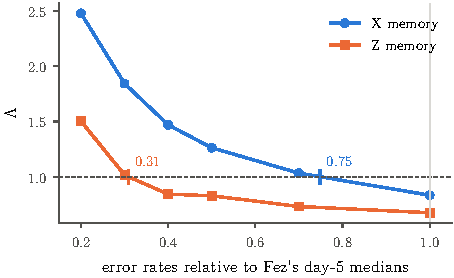
\includegraphics[width=\columnwidth]{figures/scale.pdf}
\caption{Simulated $\Lambda$ in the calibration model (no leakage, $f=1$) on a uniform chip at Fez's day-5 median error rates, with all error rates scaled together; 20,000 shots per point. Ticks mark where $\Lambda$ crosses one, interpolated between grid points.}
\label{fig:scale}
\end{figure}

%======================================================================
\begin{table*}[t]
\caption{Each repetition against the prediction at its measured $f$ (in parentheses). The \emph{Agree} columns list which of $\eps_3$, $\eps_5$ and $\Lambda$ agree with the prediction under the pre-registered bound.}
\label{tab:reps}
\footnotesize
\begin{ruledtabular}
\begin{tabular}{lcccl@{\hspace{2.5em}}cccl}
 & \multicolumn{4}{c}{X memory} & \multicolumn{4}{c}{Z memory} \\
\cline{2-5}\cline{6-9}
Day, rep. & $\eps_3$ (\%) & $\eps_5$ (\%) & $\LX$ & Agree & $\eps_3$ (\%) & $\eps_5$ (\%) & $\LZ$ & Agree \\
\hline
1, 1 & 13.2 (9.7) & 17.6 (17.9) & $0.75\pm0.07$ (0.54) & $\eps_5$ & 12.9 (6.5) & 26.6 (16.7) & $0.48\pm0.05$ (0.39) & none \\
1, 2 & 10.1 (8.1) & 22.0 (20.1) & $0.46\pm0.03$ (0.40) & all & 13.7 (8.8) & 23.3 (15.4) & $0.59\pm0.11$ (0.57) & $\eps_5$, $\Lambda$ \\
2, 1 & 11.9 (11.8) & 18.2 (14.3) & $0.65\pm0.05$ (0.82) & $\eps_3$ & 13.5 (7.0) & 32.6 (17.0) & $0.42\pm0.04$ (0.41) & $\Lambda$ \\
2, 2 & 12.0 (7.7) & 22.0 (18.3) & $0.54\pm0.04$ (0.42) & $\eps_5$, $\Lambda$ & 20.1 (8.5) & 28.0 (16.1) & $0.72\pm0.11$ (0.53) & $\Lambda$ \\
3, 1 & 13.7 (10.4) & 19.8 (16.6) & $0.69\pm0.06$ (0.63) & $\eps_5$, $\Lambda$ & 14.9 (8.2) & 23.6 (16.6) & $0.63\pm0.10$ (0.49) & $\eps_5$, $\Lambda$ \\
3, 2 & 11.1 (10.2) & 21.4 (19.0) & $0.52\pm0.04$ (0.54) & all & 14.9 (8.7) & 26.6 (16.3) & $0.56\pm0.04$ (0.54) & $\Lambda$ \\
4, 1 & 12.1 (9.7) & 17.8 (15.8) & $0.68\pm0.06$ (0.62) & all & 13.6 (7.6) & 27.9 (15.3) & $0.49\pm0.04$ (0.49) & $\Lambda$ \\
4, 2 & 10.5 (8.8) & 21.2 (19.3) & $0.49\pm0.04$ (0.45) & all & 17.0 (7.7) & 23.2 (18.3) & $0.73\pm0.11$ (0.42) & $\eps_5$ \\
5, 1 & 12.5 (9.6) & 19.1 (15.8) & $0.65\pm0.06$ (0.60) & $\eps_5$, $\Lambda$ & 13.8 (6.2) & 34.1 (17.4) & $0.40\pm0.03$ (0.35) & $\Lambda$ \\
5, 2 & 11.9 (8.2) & 23.2 (19.3) & $0.51\pm0.04$ (0.43) & $\eps_5$, $\Lambda$ & 23.6 (8.1) & 26.9 (16.3) & $0.88\pm0.10$ (0.50) & none \\
\end{tabular}
\end{ruledtabular}
\end{table*}

\section{Discussion}
\label{sec:discussion}
%======================================================================

$\Lambda$ for the heavy-hex code at distances 3 and 5 on Fez is below one in both bases, as the calibration model predicted, and varies strongly with placement: in X memory the two placements give $0.68$ and $0.50$, each stable over five days.
With only two placements, this is firm for them and suggestive for the device.

The calibration model captures the ordering of the placements and, once its own day-to-day scatter is admitted, $\LX$.
It does not capture the logical error rates.
Every unmodelled effect we can identify adds error: two-pulse decoupling leaves about echo-level dephasing, the memory runs imply more dephasing than the idle test, and the flags reveal a persistent state, consistent with leakage, that the resets do not clear and that is shared between neighbouring qubits.

Our errors per round are comparable to earlier heavy-hex experiments in X memory and higher in Z memory.
Without leakage post-selection, Ref.~\cite{sundaresan2023demonstrating} reports 11.3\% per round in X memory and 5.9\% in Z memory at distance~3 on a Falcon processor (about 3--4\% in Z memory after post-selection), against our 10--14\% and 13--24\%.
On Heron~r2, Ref.~\cite{harper2026characterising} reduced the error per round from above 10\% to 3--4\% by measuring the X and Z gauges in parallel and without resets, shortening the round from 11.1 to $3.2\us$; it attributes the gain mainly to reduced relaxation during measurement and found resets alone to make a negligible difference.
Our round spends $6.7\us$ of its $7.9\us$ on two readouts and two resets, and uses twelve CX gates per bulk Z gauge.
The readout and reset time sets the idle decay, and the persistent state is twice as frequent on flags, which undergo more gates, readouts and resets.
The natural next steps are a shorter round with parallel gauge measurements, a shorter Z gauge, resets that remove leakage~\cite{miao2023overcoming}, longer decoupling sequences, and twirled gates and readout, so that the noise is closer to the Pauli channels a stabilizer model assumes.
A calibration-based model of such circuits needs, at a minimum, a leakage term with its spread and the calibration's day-to-day scatter in its error budget; IBM's separate reset errors and outcome-resolved readout errors improve agreement at the detector level.

\paragraph*{Limitations.}
Only two distance-5 placements were available; they share 51 of 65 qubits and were the same every day.
One calibration serves all repetitions of a day, and when a repetition's patches ran in separate jobs they ran about one minute apart.
The pre-registered error bars include shot noise, the measured $f$ and recalibration during a job, but not day-to-day calibration scatter.
$\eps$ and $\Lambda$ describe one to eight rounds, not asymptotic rates; the distance-5 eight-round points lie near 50\% and drop out of the fit in four of ten repetitions in each basis, and in Z memory on two occasions the six-round point as well, leaving $\eps_5$ to rounds one to four.
The decoder's priors come from the same calibration model that the data show to be incomplete, so $\Lambda$ with a decoder calibrated on the data could be higher.
The idle test likely underestimates $f$ during memory.
The diagnosis is exploratory: its 320 readout series come from 38 physical qubits, gate and measurement counts are confounded across qubit roles, and the leakage model has an assumed form fitted to four of the fifteen jobs.

\begin{acknowledgments}
We acknowledge the use of IBM Quantum services for this work.
The views expressed are those of the author and do not reflect the official policy or position of IBM or the IBM Quantum team.
The circuits, simulations, placement and analysis code were written with the AI assistants Claude (Anthropic) and Cursor (including xAI's Grok models), which also helped edit the text, and the exploratory diagnosis was carried out with AI assistance at the author's direction.
The author designed the experiment, checked the code and results, and takes responsibility for the content.
\end{acknowledgments}

\paragraph*{Data availability.}
The data that support the findings of this article are openly available~\cite{repo}: every job's calibration, compiled circuits, predictions, shots and analysis, the code that produced them, the diagnosis scripts and results, and the scripts that draw the figures.

%======================================================================
\appendix
%======================================================================

\section{Pre-registration record}
\label{app:record}

The repository's history before the experiment was rewritten twice by force-pushes (24 September and 2 October 2026; the second changed only one commit message); from 3 October onward it matches GitHub's log of pushes.
On 3 October two single-job designs were released (v0.1.0 and v0.1.1) and then replaced by a design with several days and up to two repetitions a day under a 300\,s budget.
A folder prepared for the single-job design was deleted without being submitted; no QPU data were taken before the first job of the experiment.
The final design (commit \texttt{1c86fce}) and pooling rule (\texttt{cd4a68e}) were committed 31 and 13 minutes before the first job, at 21:33~UTC on 3 October, and released as v0.2.0 at 21:29~UTC and archived by Zenodo~\cite{zenodo}; the archive matches that commit file for file.
Days 2--5 were not released separately.
Their record is the git history together with GitHub's log of pushes, which shows each day's folder pushed 14--15\,s before that day's first submission (8~min on day~1), and the IBM job identifiers, whose embedded timestamps match the recorded submission times.
On day~2 the folder was prepared twice, because IBM published a new calibration between preparation and submission; only the calibration's timestamp changed, and the predictions were identical.
Days 2--5 were prepared and submitted by a script added after day~1, which runs the unchanged submission code with the same per-job and total QPU limits.
No copy of the manuscript text was archived before the run; the design and decision rules it describes are those of the code as released.
The code and its configuration are unchanged from \texttt{cd4a68e} to the end of the experiment, and every job records the same code hash.

\section{Statistical procedures and per-repetition results}
\label{app:stats}

\paragraph*{Fit.}
$\mathrm{Var}(\eps)$ is scaled by the reduced $\chi^2$ of the fit when it exceeds one and propagated to $\Lambda$ as $\mathrm{Var}(\Lambda)/\Lambda^2 = \mathrm{Var}(\eps_3)/\eps_3^2 + \mathrm{Var}(\eps_5)/\eps_5^2$.
At one to eight rounds a single $\eps$ is an approximation: in simulation of repetition~1 on day~1 the fit has reduced $\chi^2 = 12.6$ for distance-5 X memory at $f=0$, and $A \approx 1.04$ in distance-3 Z memory.
Omitting the one-round point changes the predicted $\LX$ by 0.01; prediction and data are fitted identically.
As an exploratory check, $\LX$ from rounds 2--8 is 0.88, 0.67, 0.62, 0.64 and 0.78 for repetition~1 on days 1--5 (predicted 0.53, 0.82, 0.62, 0.61, 0.60) and 0.51, 0.61, 0.55, 0.62 and 0.46 for repetition~2 (predicted 0.39, 0.42, 0.54, 0.44, 0.42), each $\pm 0.1$.

\paragraph*{Power.}
In simulation of these fits at 2500 shots per circuit, a single repetition's $\LX$ has a standard error of about 0.03.
A pooled $\LX$ of exactly one is declared different from one in 2--6\% of simulated experiments with shot noise alone, 7--20\% with twice that scatter and up to 41\% with four times; at the predicted $\LX$ every simulated experiment declares distance~5 worse.
If the model is exactly right, the three correlated experiment-level agreement tests together fail in 6--12\% of simulated experiments, and the $\LX$ test detects a mismatch of 0.04--0.06 in every repetition with 80\% probability.

\paragraph*{Agreement bound.}
The predicted variance combines simulator shot noise; the uncertainty in $f$ times the quantity's slope in $f$, from the predictions at $f=0$, the measured $f$ and $f=1$, or from the line through $f=0$ and $f=1$ when the measured $f$ lies within 0.05 of either end or beyond it (nine of the fifteen jobs); and $\Delta^2/2$, where $\Delta$ is the difference between predictions from the calibrations before and after the job ($\Delta = 0$ throughout).

\paragraph*{Other estimators.}
Pooling $\ln\LX$ instead of $\LX$ gives $0.58\pm0.03$, and the unweighted mean of the repetitions $0.60\pm0.03$; inverse-variance pooling of a ratio is biased low because a smaller $\Lambda$ has a smaller error.

\paragraph*{Anomalous detectors.}
A detector is counted as anomalous if it fires above prediction by more than $\sqrt{2\ln N}$ standard errors, $3.81$ for the $N = 1428$ detectors of a two-patch job; for independent detectors the largest excess has median 3.3 and exceeds this bar in about 9\% of jobs.

\paragraph*{Per-repetition results.}
Table~\ref{tab:reps} lists every repetition.


\section{\texorpdfstring{Measuring $f$}{Measuring f}}
\label{app:f}

For each data qubit, $r(n) = \sqrt{\langle X\rangle^2 + \langle Y\rangle^2}$ after $n$ idle rounds decays through dephasing alone.
We fit $\ln r(n) = a + \ln x_0(n) - f\,[\ln x_0(n) - \ln x_1(n)]$ by weighted least squares, where $x_0$ and $x_1$ are the simulated $\langle X\rangle$ at $f = 0$ and $1$ and $a$ absorbs readout error; $\langle X\rangle^2 + \langle Y\rangle^2$ is corrected for shot noise, and points with $r \le 0.05$ are dropped.
Negative estimates are set to zero, qubits whose $f$ cannot be determined to $\pm0.5$ are excluded, and the median over data qubits is used, with standard error 1.25 times that of the mean.
Across all jobs the interquartile range over qubits is 0.46--1.53, and the inverse-variance mean (0.02--0.59) is biased low because larger values of $f$ are measured less precisely (Spearman $\rho = 0.77$ between $f$ and its uncertainty).

\bibliography{refs}

\end{document}
